\documentclass[10pt,brazil,english]{article}
\usepackage{amsfonts}
\usepackage{infocomp}
\usepackage{times}
\usepackage{amsmath}
\usepackage{amssymb}
\usepackage[T1]{fontenc}
\usepackage[english, portuguese]{babel}
\addto\captionsportuguese{
\renewcommand{\figurename}{Figura}
\renewcommand{\tablename}{Tabela}
\renewcommand{\refname}{REFER\^{E}NCIAS}
}
\usepackage[utf8]{inputenc}
\usepackage{multirow}
\usepackage{lscape}
\usepackage{rotating}
\usepackage{setspace} % espacamento entre linhas
\usepackage[table,xcdraw]{xcolor}
\usepackage{scalefnt}
\usepackage{graphicx}
\usepackage{hyperref}
\usepackage{subfigure}
\usepackage{enumerate}
\usepackage{caption}
\usepackage[sort,compress]{cite}
\usepackage[alf,abnt-repeated-author-omit=yes,abnt-etal-list=0]{abntex2cite}	% Citações padrão ABNT
%%%%%%%%%%%%%%%%%%%%%%%%%%%%%%%%%%%%%%%%%%%%%%%%%%%%%%%%%
\usepackage{fancyhdr}
\usepackage{mathtools}
\usepackage{icomma}
\setcounter{page}{1}
\fancyhead{ }
\lhead{}
\chead{\footnotesize ANÁLISE E IMPLEMENTAÇÃO DE MODELOS ESTOCÁSTICOS PARA EVOLUÇÃO DE ESPÉCIES}
\rhead{}
\cfoot{}
\rfoot{\thepage}%Direita do Rodapé
\renewcommand{\headrulewidth}{1pt}% Traço horizontal no cabeçalho

%%%%%%%%%%%%%%%%%%%%%%%%%%%%%%%%%%%%%%%%%%%%%%%%%%%%%%%%%

\usepackage{rangecite}

%\hyphenation{po-pu-la-ri-za-ção re-gis-tros do-mi-na-do-ra vio-la pe-ram-bu-lam dou-tri-na-ria-men-te co-nhe-ce-rem Ad-mis-tra-ção fa-bri-car so-cie-da-de in-fe-rio-res vee-men-te-men-te si-tua-ção pon-tuais}

\sloppy
\renewcommand{\captionfont}{\footnotesize}
\renewcommand{\captionlabelfont}{\footnotesize \bfseries}
\title{ANÁLISE E IMPLEMENTAÇÃO DE MODELOS ESTOCÁSTICOS PARA EVOLUÇÃO DE ESPÉCIES}

\address{
$^{1}$Fundação Getulio Vargas (FGV)}

\author{Lucas Emanuel Resck Domingues$^{1}$}

\selectlanguage{english}

\abstract{
    This work presents some stochastic models for species evolution: the Bak-Sneppen model \cite{bak1993punctuated} and the GMS model \cite{guiol2009stochastic}, both studied by \citeonline{khouri2013estudos}.
    Important evolutionary concepts for the discussion of these models are presented, such as natural selection.
    The models are discrete and work with species adaptation degrees (fitnesses) for natural selection.
    Implementations of simulation with Python language are performed, and fitnesses distributions graphics are obtained.
    It's suggested or demonstrated that these distributions converge in these models, and the simulation results are used as verification.
    The latter is done from the graphics and the hypothesis testing of the parameters of the distributions.
    Advantages and conceptual errors of the models are discussed.
}

\keywords{Evolution. Natural Selection. Python. Stochastic Models.}

\selectlanguage{brazil}

\resumo {
    Este trabalho apresenta alguns modelos estocásticos para evolução de espécies: o modelo introduzido por \citeonline{bak1993punctuated} e o modelo introduzido por \citeonline{guiol2009stochastic}, ambos estudados por \citeonline{khouri2013estudos}.
    São apresentados conceitos evolutivos importantes para a discussão desses modelos, como seleção natural.
    Os modelos são discretos e trabalham com graus de adaptação das espécies (\textit{fitnesses}) para a seleção natural.
    Implementações de simulações utilizando a linguagem \textit{Python} são realizadas, e gráficos das distribuições dos \textit{fitnesses} são obtidos.
    É sugerido ou demonstrado que essas distribuições convergem nesses modelos, e os resultados das simulações são utilizados como verificação.
    Esta se dá a partir dos gráficos e de testes de hipóteses do parâmetro da distribuição.
    Vantagens e erros conceituais dos modelos são discutidos.
}

\palchaves{Evolução. Seleção Natural. \textit{Python}. Modelos Estocásticos.}

\begin{document}
    \pagestyle{fancy} % CABECALHOO
    
    \maketitle
    \newpage

    \newtheorem{theorem}{Teorema}
    
    \section{INTRODUÇÃO}

        A Evolução é uma das teorias mais sofisticadas da Biologia, principalmente pela sua simplicidade algorítmica.
        Desde o início da busca pelo conhecimento, os seres humanos tentaram entender a origem dos seres vivos.
        A Teoria Evolutiva diz que os seres vivos surgiram todos de um ancestral comum, que se modificou ao longo do tempo, por diversos fatores.
        
        A seleção natural talvez seja o mecanismo mais forte da Teoria Evolutiva.
        Basicamente é um algoritmo que seleciona os indivíduos melhor adaptados para que se reproduzam e perpetuem suas características.
        \citeonline{khouri2013estudos} exemplica com bactérias. Suponhamos que, em uma placa de Petri, haja uma colônia de bactérias suficientemente já desenvolvida (com milhões de indivíduos).
        Despejamos um antibiótico nessa placa e, após certo tempo, observamos que algumas bactérias sobreviveram e se reproduziram.
        Essa "nova colônia" \space agora é resistente a esse antibiótico.
        Isso se deve ao fato de que existiam bactérias na colônia inicial que eram resistentes ao componente.
        Quando o despejamos, selecionamos aqueles indivíduos resistentes, que se reproduziram e passaram essa característica de resistência adiante.

        Dessa forma, este trabalho tem como objetivos analisar e simular ambientes de seleção natural propostos por \citeonline{bak1993punctuated} e \citeonline{guiol2009stochastic}.
        Na verdade, ele foi inspirado na dissertação de \citeonline{khouri2013estudos}, que estuda e compara esses modelos.
        São modelos discretos simples de seleção natural, mas com algumas implicações sobre as distribuições dos graus de adaptação (\textit{fitnesses}).

        Na seção 2, apresento o modelo que chamarei de Bak-Sneppen e a sugestão do autor de convergência da distribuição dos \textit{fitnesses}.
        Na seção 3, apresento o modelo GMS, além de um teorema forte apresentado pelos autores.
        A seção 4 introduz a implementação da simulação dos modelos.
        Na seção 5, apresento gráficos das distribuições obtidas pelas simulações.
        
        As discussões dos resultados e de conceitos se dão na seção 6.
        Os modelos são interpretados, assim como seus resultados.
        Além disso, são testadas hipóteses relativas aos parâmetros das distribuções dos \textit{fitnesses}.
        Ao final, erros conceituais dos modelos são discutidos, principalmente no que diz respeito a equilíbro pontuado e gradualismo.

        Este é um trabalho avaliado para a disciplina Modelagem de Fenômenos Biológicos, ministrada por Claudio Struchiner, da Escola de Matemática Aplicada da Fundação Getulio Vargas.
    
    \section{MODELO BAK-SNEPPEN}

        \citeonline{bak1993punctuated} introduziram o modelo que chamarei de Bak-Sneppen.
        Seu funcionamento é descrito de forma direta por \citeonline{khouri2013estudos}:

        \renewcommand{\theenumi}{\roman{enumi}} 
        \begin{enumerate}
            \item $N$ espécies são distribuídas em um grafo circular;
            \item A cada espécie é associado um número, chamado \textit{\textbf{fitness}}, que é uma amostra de uma distribuição uniforme em $[0, 1]$;
            \item Em cada "rodada", o indivíduo com o menor \textit{fitness} tem seu número sorteado novamente;
            \item O mesmo se repete para seus dois vizinhos.
        \end{enumerate}

        O modelo é relativamente simples, e no artigo é sugerido que a distribuição dos \textit{fitnesses} converge para uma uniforme em $(f^*, 1]$, com $f^* \approx 2/3$.

    \section{MODELO GMS}

        \citeonline{guiol2009stochastic} se basearam no modelo Bak-Sneppen para criar outro modelo, que \citeonline{khouri2013estudos} chama de GMS (as iniciais dos autores). Chamaremos assim neste trabalho. Ele é descrito:

        \renewcommand{\theenumi}{\roman{enumi}} 
        \begin{enumerate}
            \item O modelo é discreto e se inicia no conjunto vazio;
            \item A cada etapa do processo, uma espécie nasce (com probabilidade $p$) ou uma espécie morre (com probabilidade $q = 1 - p$) (se o conjunto de espécies é vazio, ele se mantém constante);
            \item Cada espécie tem associada a si um número \textit{fitness} amostrado de uma uniforme $[0, 1]$;
            \item Quando uma espécie morre, a escolhida é aquela com menor \textit{fitness} para morrer.
        \end{enumerate}

        Os autores apresentam alguns resultados. Seja $p$ tal que $p \in (1/2, 1)$ e tomemos $$f_c = \frac{1 - p}{p}\textrm{.}$$
        Então $f_c \in (0, 1)$.
        Vamos representar as espécies a partir do seu \textit{fitness}.
        Consideremos $L_n$ e $R_n$ as espécies que estão vivas no tempo $n$ que são menores e maiores que $f_c$, respectivamente. Ou seja, $L_n \subseteq (0, f_c)$ e $R_n \subseteq (f_c, 1)$. A notação $|A|$ indica a cardinalidade de $A$. Então:

        \begin{theorem} \cite{guiol2009stochastic}
            \label{theorem1}
            \renewcommand{\theenumi}{\alph{enumi}} 
            \begin{enumerate}
                \item $|L_n|$ é uma cadeia de nascimento-morte recorrente nula. Em particular, $L_n$ é vazio infinitas vezes com probabilidade um.
                \item Se $f_c < a < b < 1$, então $$\lim_{n \to \infty} \dfrac{1}{n} |R_n \cap (a, b)| = p(b - a) \textrm{.}$$
            \end{enumerate}
        \end{theorem}

        São resultados muito fortes, porém \citeonline{guiol2009stochastic} resumem dizendo que assintoticamente a distribuição das espécies se dá uniformemente em $(f_c, 1)$.

    \section{IMPLEMENTAÇÃO}

        A implementação dos modelos foi realizada em \textit{Python} e os resultados foram visualizados em \textit{Jupyter Notebook} \cite{domingues2019github}.

        O objetivo desta etapa é verificar os resultados apresentados que dizem respeito à convergência das distribuições dos \textit{fitnesses}.

    \section{RESULTADOS}

        \subsection{Modelo Bak-Sneppen}

            O algoritmo implementado para o modelo foi executado com 2000 espécies por 1 milhão de iterações.
            A Figura \ref{Fig1} mostra um histograma dos \textit{fitnesses}.

            \begin{figure}[!hbtp]
                \begin{center}
                    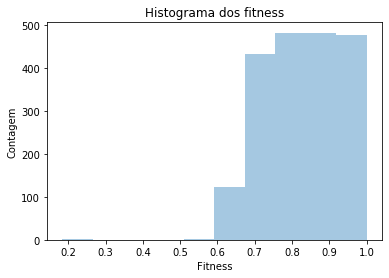
\includegraphics[scale=0.5]{Images/5-1.png}
                \end{center}
                \caption{Histograma dos \textit{fitnesses} para 2000 espécies em um milhão de iterações.}
                \label{Fig1}
            \end{figure}

        \subsection{Modelo GMS}

            O algoritmo implementado para o modelo foi executado com cem mil iterações.
            A Figura \ref{Fig2} mostra um histograma dos \textit{fitnesses} quando $p = 2/3$, e a Figura \ref{Fig3}, quando $p = 3/5$.

            \begin{figure}[!hbtp]
                \begin{center}
                    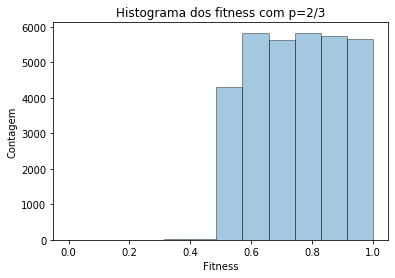
\includegraphics[scale=0.5]{Images/5-2-1.png}
                \end{center}
                \caption{Histograma dos \textit{fitnesses} para $p = 2/3$ em cem mil iterações.}
                \label{Fig2}
            \end{figure}

            \begin{figure}[!hbtp]
                \begin{center}
                    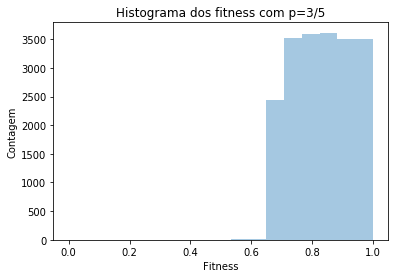
\includegraphics[scale=0.5]{Images/5-2-2.png}
                \end{center}
                \caption{Histograma dos \textit{fitnesses} para $p = 3/5$ em cem mil iterações.}
                \label{Fig3}
            \end{figure}            

    \section{DISCUSSÕES}

        Ambos os modelos tentam aproximar um processo de evolução por seleção natural.
        O modelo de Bak-Sneppen dispõe as espécies em um grafo, como uma tentativa de representar uma interação entre as espécies, como predação e comensalismo \cite{khouri2013estudos}.
        A cada rodada, a espécie menos adaptada é eliminada, de modo que surge outra espécie com \textit{fitness} aleatório, ou seja, o número de espécies é fixo.
        O mesmo acontece para seus dois vizinhos.
        E o processo se repete.

        O modelo GMS adota um número de espécies variável, mas não considera interação entre as espécies (ou seja, os vizinhos não morrem juntos).
        A não ser por essas considerações, o modelo funciona de maneira parecida: espécies surgem com \textit{fitness} aleatório e aquelas menos adaptadas morrem.

        A Figura \ref{Fig1} mostra um histograma próximo daquele de uma distribuição uniforme em $(2/3, 1]$, como é sugerido por \citeonline{bak1993punctuated}.
        Vamos realizar um teste da nossa hipótese.
        Nas simulações realizadas, obtivemos uma distribuição.
        Vamos amostrar dessa distribuição, supondo que ela seja uniforme em $(f_c, 1]$.
        Ou seja, tomamos uma amostra aleatória $X_1, \cdots, X_{50}$, com $X_i \sim u(f_c, 1]$ para $i = 1, \cdots, 50$.
        Sejam as hipóteses:

        \begin{equation}
            \label{eq1}
            \begin{aligned}
                H_0&: f_c = 2/3, \\
                H_1&: f_c \neq 2/3
            \end{aligned}
        \end{equation}

        Seja $Y = \min_{i = 1, \cdots, 50}(X_i)$. Rejeito $H_0$ se $Y \notin (2/3 - c, 2/3 + c)$.
        Para um teste nível $\alpha_0 = 0,05$, calculo $c = 0,019$.

        O teste foi realizado para a distribuição apresentada na Figura \ref{Fig1}.
        Foi observado $y = 0,656$ e $H_0$ não foi rejeitada.

        A Figura \ref{Fig2} mostra um histograma próximo daquele de uma distribuição $(1/2, 1]$. Observe que $p = 2/3$.
        O Teorema \ref{theorem1} nos diz que, no limite, a distribuição das espécies é $(f_c, 1)$, com $f_c = (1 - 2/3)/(2/3) = 1/2$.
        Ora, é isso que observamos. Vamos testar essa hipótese.
        Tomamos uma amostra aleatória $X_1, \cdots, X_{50}$, com $X_i \sim u(f_c, 1]$ para $i = 1, \cdots, 50$.
        Sejam as hipóteses:

        \begin{equation}
            \label{eq2}
            \begin{aligned}
                H_0&: f_c = 1/2, \\
                H_1&: f_c \neq 1/2
            \end{aligned}
        \end{equation}

        Seja $Y = \min_{i = 1, \cdots, 50}(X_i)$. Rejeito $H_0$ se $Y \notin (1/2 - c, 1/2 + c)$.
        Para um teste nível $\alpha_0 = 0,05$, calculo $c = 0,029$.

        O teste foi realizado para a distribuição apresentada na Figura \ref{Fig2}, em que $p = 2/3$.
        Foi observado $y = 0,493$ e $H_0$ não foi rejeitada.

        Análogo à Figura \ref{Fig2}, a Figura \ref{Fig3} aproxima uma distribuição uniforme em $(2/3, 1]$, o que é esperado para valor $p = 3/5$ considerado.
        Vamos testar essa hipótese.
        Observe que estamos lidando com a mesma distribuição do caso para o modelo Bak-Sneppen e as mesmas hipóteses de \ref{eq1}.
        Dessa forma, o teste é o mesmo.

        Foi observado $y = 0,672$ e $H_0$ não foi rejeitada.

        As simulações e os testes de hipóteses reforçam o que esperar das distribuições dos \textit{fitnesses} das espécies para cada um dos modelos.

        Os modelos apresentados e testados possuem a vantagem de ser suficientemente simples (ao ponto de serem didáticos), em que evolução e seleção natural são resumidas em poucos passos de um algoritmo bem direto.
        Porém, toda essa simplicidade e didática refletem, de certa forma, erros conceituais importantes no estudo biológico.

        \citeonline{khouri2013estudos} aponta que ambos os modelos se baseiam na ideia do equilíbrio pontuado.
        Esta é uma teoria evolutiva que modela a evolução não de um ponto de vista gradual, mas através de "saltos".
        Ou seja, longos períodos sem grandes mutações e pequenos períodos com muita variação.
        Isso é refletido principalmente ao se observar registros fósseis, que podem apresentar esse tipo de padrão \cite{khouri2013estudos}.

        Porém, atualmente o equilíbrio pontuado já não é mais tanto aceito, e a teoria predominante é a do gradualismo, em que a evolução ocorre de forma gradual.
        Inclusive é possível obter registros fósseis que apresentem evolução gradual \cite{khouri2013estudos}.

        Ambos os modelos trabalham a seleção natural no nível das espécies, ou seja, espécies são selecionadas.
        Porém, \citeonline{khouri2013estudos} ressalta que atualmente já é bastante aceito que isso não acontece, e que a seleção natural, na verdade, acontece no nível dos genótipos.

    \bibliography{Referencias}
    
\end{document} 